\chapter{Systembeskrivelse}
\section{Systembeskrivelse}
Formålet med dette projekt er at udvikle en invasiv blodtryksmåler, der skal være på en operationsstue. Den invasive blodtryksmåler er et system, der har til formål at kunne måle, angive og visualisere en patients systolisk-, diastolisk og middelblodtryk samt puls. Blodtrykket visualiseres kontinuert, når det tilsluttes det væskefyldte kateter. Derudover vil systemet alarmere i visse situationer beskrevet i punkt 2.2.
Systemet består af en hardware del og en software del. 


Systemets software del skal udvikle et program, der skal kunne kalibrere, vise blodtrykket kontinuerligt, måle puls og gemme de målte data. Derudover skal programmet indeholde et digital filter til filtrering af boldtrykket. Det digitale filter skal kunne slås til og fra. Programmet er bygget op omkring et Graphical User Interface (GUI) bestående af følgende elementer:
\vspace{0.7 cm}

\begin{enumerate}[2.1.]
	\item Knap “Lav nulpunktsjustering” - Laver nulpunktsjustering
	\item Knap “Start” - Påbegynder målingen
	\item Knap “Indstil grænseværdi” - Gør det muligt at ændre på grænseværdier under en måling eller før en måling Pr. deafult er der valgt flg. værdier: 
	Puls øvre: 120
	Puls nedre: 60
	Blodtrykkets øvre grænseværdi er værdien for det systoliske blodtryk. Dette er valgt til 160. 
	Blodtrykkets nedre grænseværdi er værdien for det diastoliske blodtryk. Dette er valgt til 60 
	\item Knap “Ryd” - Rydder alle værdier på brugergrænsefladen
	\item Knap “Stop” - Stopper målingen.
	\item Knap “Gem” - Gemmer værdier for blodtryksmåling, alarmer, digitaltfilter, patientens CPR og brugerens ID.
	\item Knap “Kalibrering” - Kalibrerer systemet.
	\item Knap “Mute alarm” - Gør alarm lydløs. De visuelle effekter vil stadig være synlige.
	\item Knap “Afbryd alarm” - Stopper en alarm.
	\item To radiobuttons - Slår digitalt filter til eller fra. Er monitor valgt er filteret aktiveret. Er mode valgt er filteret deaktiveret. Monitor valgt pr. default. 
	\item Tekstbokse - Indeholder data I form af systolisk-, diastolisk-, middelblodtryk og puls. 
	\item Chart - Indeholder kontinuert graf over patientens blodtryk
\end{enumerate}

\vspace{0.7 cm}
Se også punkt 2.3 “Skitse af brugergrænseflade”


Systemets hardware består af et elektrisk kredsløb der skal kunne forstærke blodtrykssignalet fra en tryktransducer. Før signalet sendes til en AD-converter filtreres det af et analogt antialiaseringsfilter. AD-converterens funktion er at konvertere det analoge signal til et digitalt signal, som vores software kan analysere.

Blodtrykket måles invasivt hvilket betyder, at blodtryksmåleren er tilsluttet patientens arterier via et væskefyldt kateter. Tryktransduceren har en membran, som registrerer trykket vha. stræk modstande. Dog vil vi i vores praktiske situation bruge en væskesøjle til at agere som patient. 


Når systemets opsætning er klart, trykkes der på “start”-knappen, som igangsætter signalvejen gennem hardwaren og ind på GUI'en. Herpå vil talværdierne svarende til patients værdier blive præsenteret. Sker der et fald i blodtrykket, f.eks. I forbindelse med en operation, vil systemet registrere dette, og starte en alarm, således brugeren gøres opmærksomme på et fald i blodtrykket. Alarmen startes, når blodtrykket falder under eller overstiger grænseværdierne, hvor det diastoliske blodtryk er den nedre grænseværdi, og det systoliske blodtryk er den øvre grænseværdi.  


Brugeren kan stoppe alarmen eller slå lyden fra alarmen, samt stoppe målingen. Efter brugeren har foretaget en blodtryksmåling, gemmes blodtryksmålingens værdier, patientens CPR-nummer, digitalt filter, alarmer og brugerens ID-nummer.
\vspace{0.9 cm}
\section{Beskrivelse af alarmer}

Systemet skal i henhold til standard 60601-1-8 kunne alarmere ved eventuelle ændringer i blodtryk samt puls. Systemet findes i operationsstuer og brugsscenariet vil derfor typisk være i forbindelse med operationer. Systemet skal alarmere ved:

\begin{enumerate}[2.2.1]
	\item Fald eller stigning i blodtryk ud over de justerbare grænseværdier
	\item Fald eller stigning i puls ud over de justerbare grænseværdier
\end{enumerate}

Alarm 2.2.1 er kategoriseret “high priority” og skal alarmere i henhold til dokumentet “Standard 60601-1-8”. Den er kategoriseret high idet det er livsfarligt for patienten, hvis der ikke handles med det samme.

Alarm 2.2.2 er kategoriseret “high priority” og skal alarmere i henhold til dokumentet “Standard 60601-1-8”. Den er kategoriseret high idet det er livsfarligt for patienten, hvis der ikke handles med det samme.

\clearpage
\section{Systemoversigt}

	\begin{figure}[h!]
	\centering
	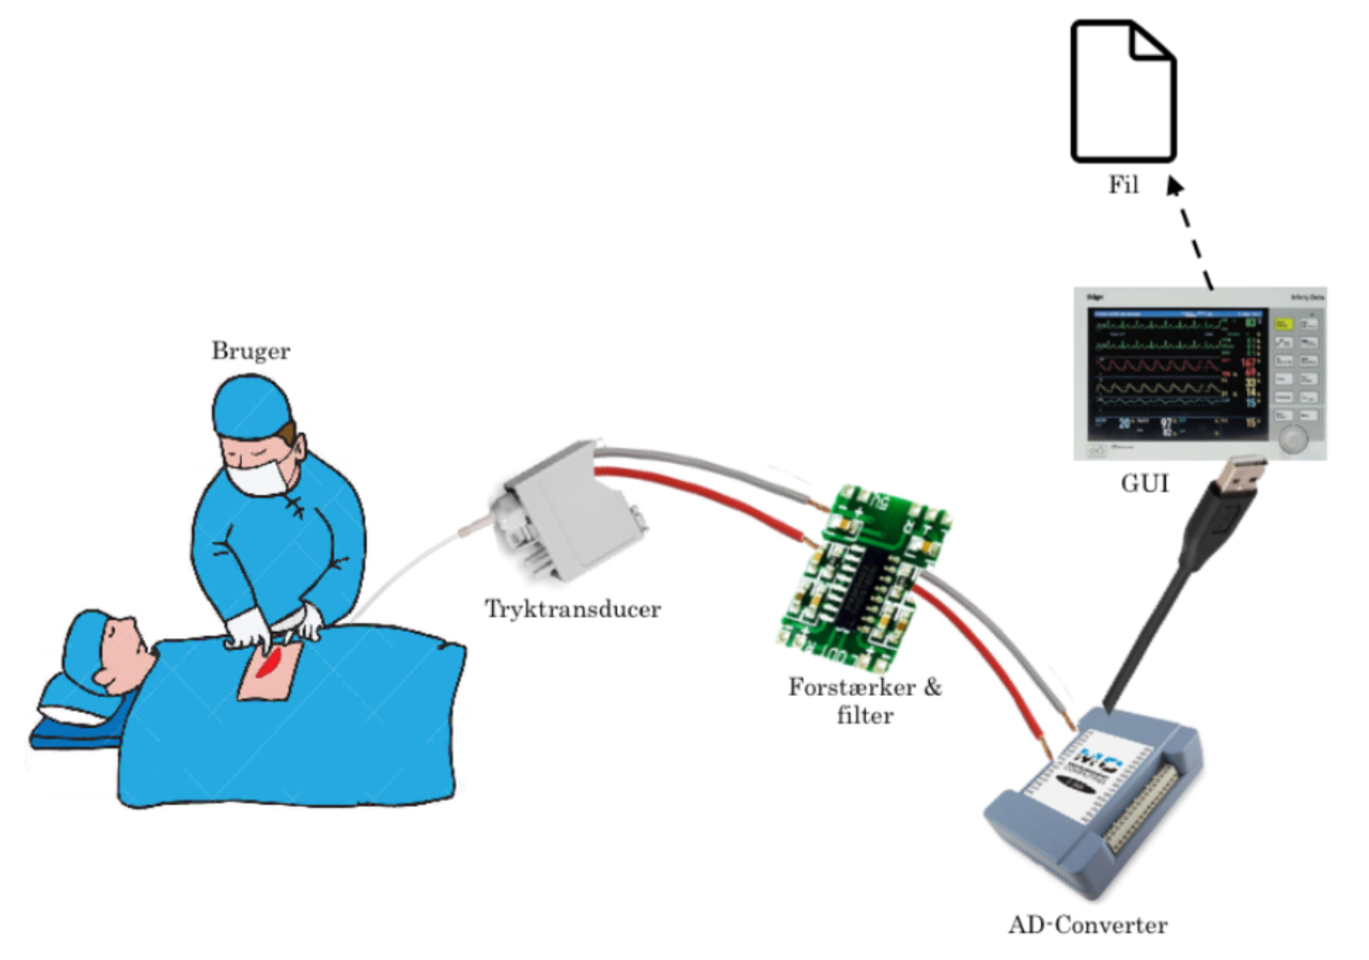
\includegraphics[width=0.55\linewidth]{Systembeskrivelse/Systemoversigt}
	\caption{Systemoversigt}
	\label{fig:Systemoversigt}
\end{figure}
\vspace{1 cm}

På figur \ref{fig:Systemoversigt} ses systemoversigten for vores blodtrykmålersystem, der har til formål at kunne måle og vise en patients blodtryk og puls på en brugergrænseflade. 

\vspace{1.5 cm}
\section{Skitse af brugergrænseflade}
\vspace{0.7 cm}
\begin{figure}[h!]
	\centering
	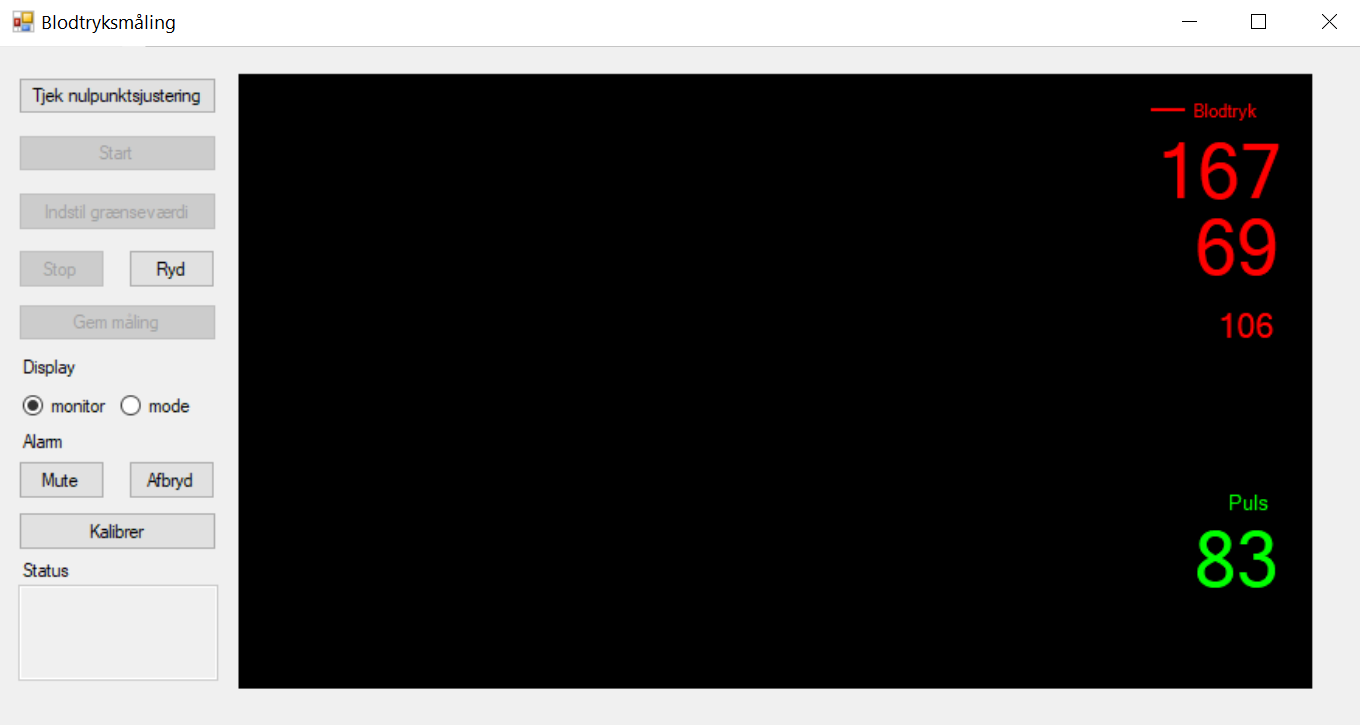
\includegraphics[width=0.7\linewidth]{Systembeskrivelse/Brugergraenseflade}
	\caption{Skitse af brugergrænseflade}
	\label{fig:Brugergraenseflade}
\end{figure}

\clearpage